
%%%%%%%%%%%%%%%%%%%%%%%%%%%%%%%%%%%%%%%%%%%%%%
%%%%%%%%          Schematics          %%%%%%%%
%%%%%%%%%%%%%%%%%%%%%%%%%%%%%%%%%%%%%%%%%%%%%%








\section{Circuitry}\label{02Sec:Circuitry}




\subsection{Block Diagram}\label{02Sub:BlockDiagram}


The block diagram of the device on the Figure \ref{02fig:BD} consists of several main components that play essential roles in its operation. 
Here is a brief overview of each of these parts:

\begin{itemize}
    \item Microcontroller (ESP8266EX): The ESP8266EX microcontroller is the central component of the device. It is responsible for 
    controlling all operations and functionalities, including wireless communication via WiFi.
    
    \item Program Memory (MX25R3235F): The program memory is where the device's firmware is stored. 
    % In this project, the MX25R3235F 
    % chip with a capacity of 32Mbit was selected. This memory stores the program that controls the device's operation, allowing it 
    % to perform the desired tasks.

    \item Data Memory (AT25SF081): The data memory is used to store the collected data in the device.
    % For this purpose, the 
    % AT25SF081 chip with a capacity of 8Mbit was chosen. This memory is utilized to store the temperature information collected 
    % by the sensor, enabling access and utilization of the data as needed.
    
    \item Temperature Sensor (TMP35): The TMP35 temperature sensor measures the ambient temperature.
    % It was chosen for its low 
    % power consumption, the ability to power off when not in use, good accuracy, and compatibility with other widely used 
    % components in the market, such as the LM35. The temperature sensor provides temperature data that is processed and stored by 
    % the device.

    \item RF Antenna (Texas SWRA117D 2.4GHz - Left): The RF antenna plays a crucial role in the wireless communication of the device. It enables 
    the transmission and reception of radio signals, allowing WiFi communication. The RF antenna ensures a stable and reliable connection between 
    the device and the access point (AP), facilitating the transmission of collected data. More information on this type of PCB antenna can be 
    found at \cite{TexasRFAntenna}.

\end{itemize}


\begin{figure}[H]
    \centering
    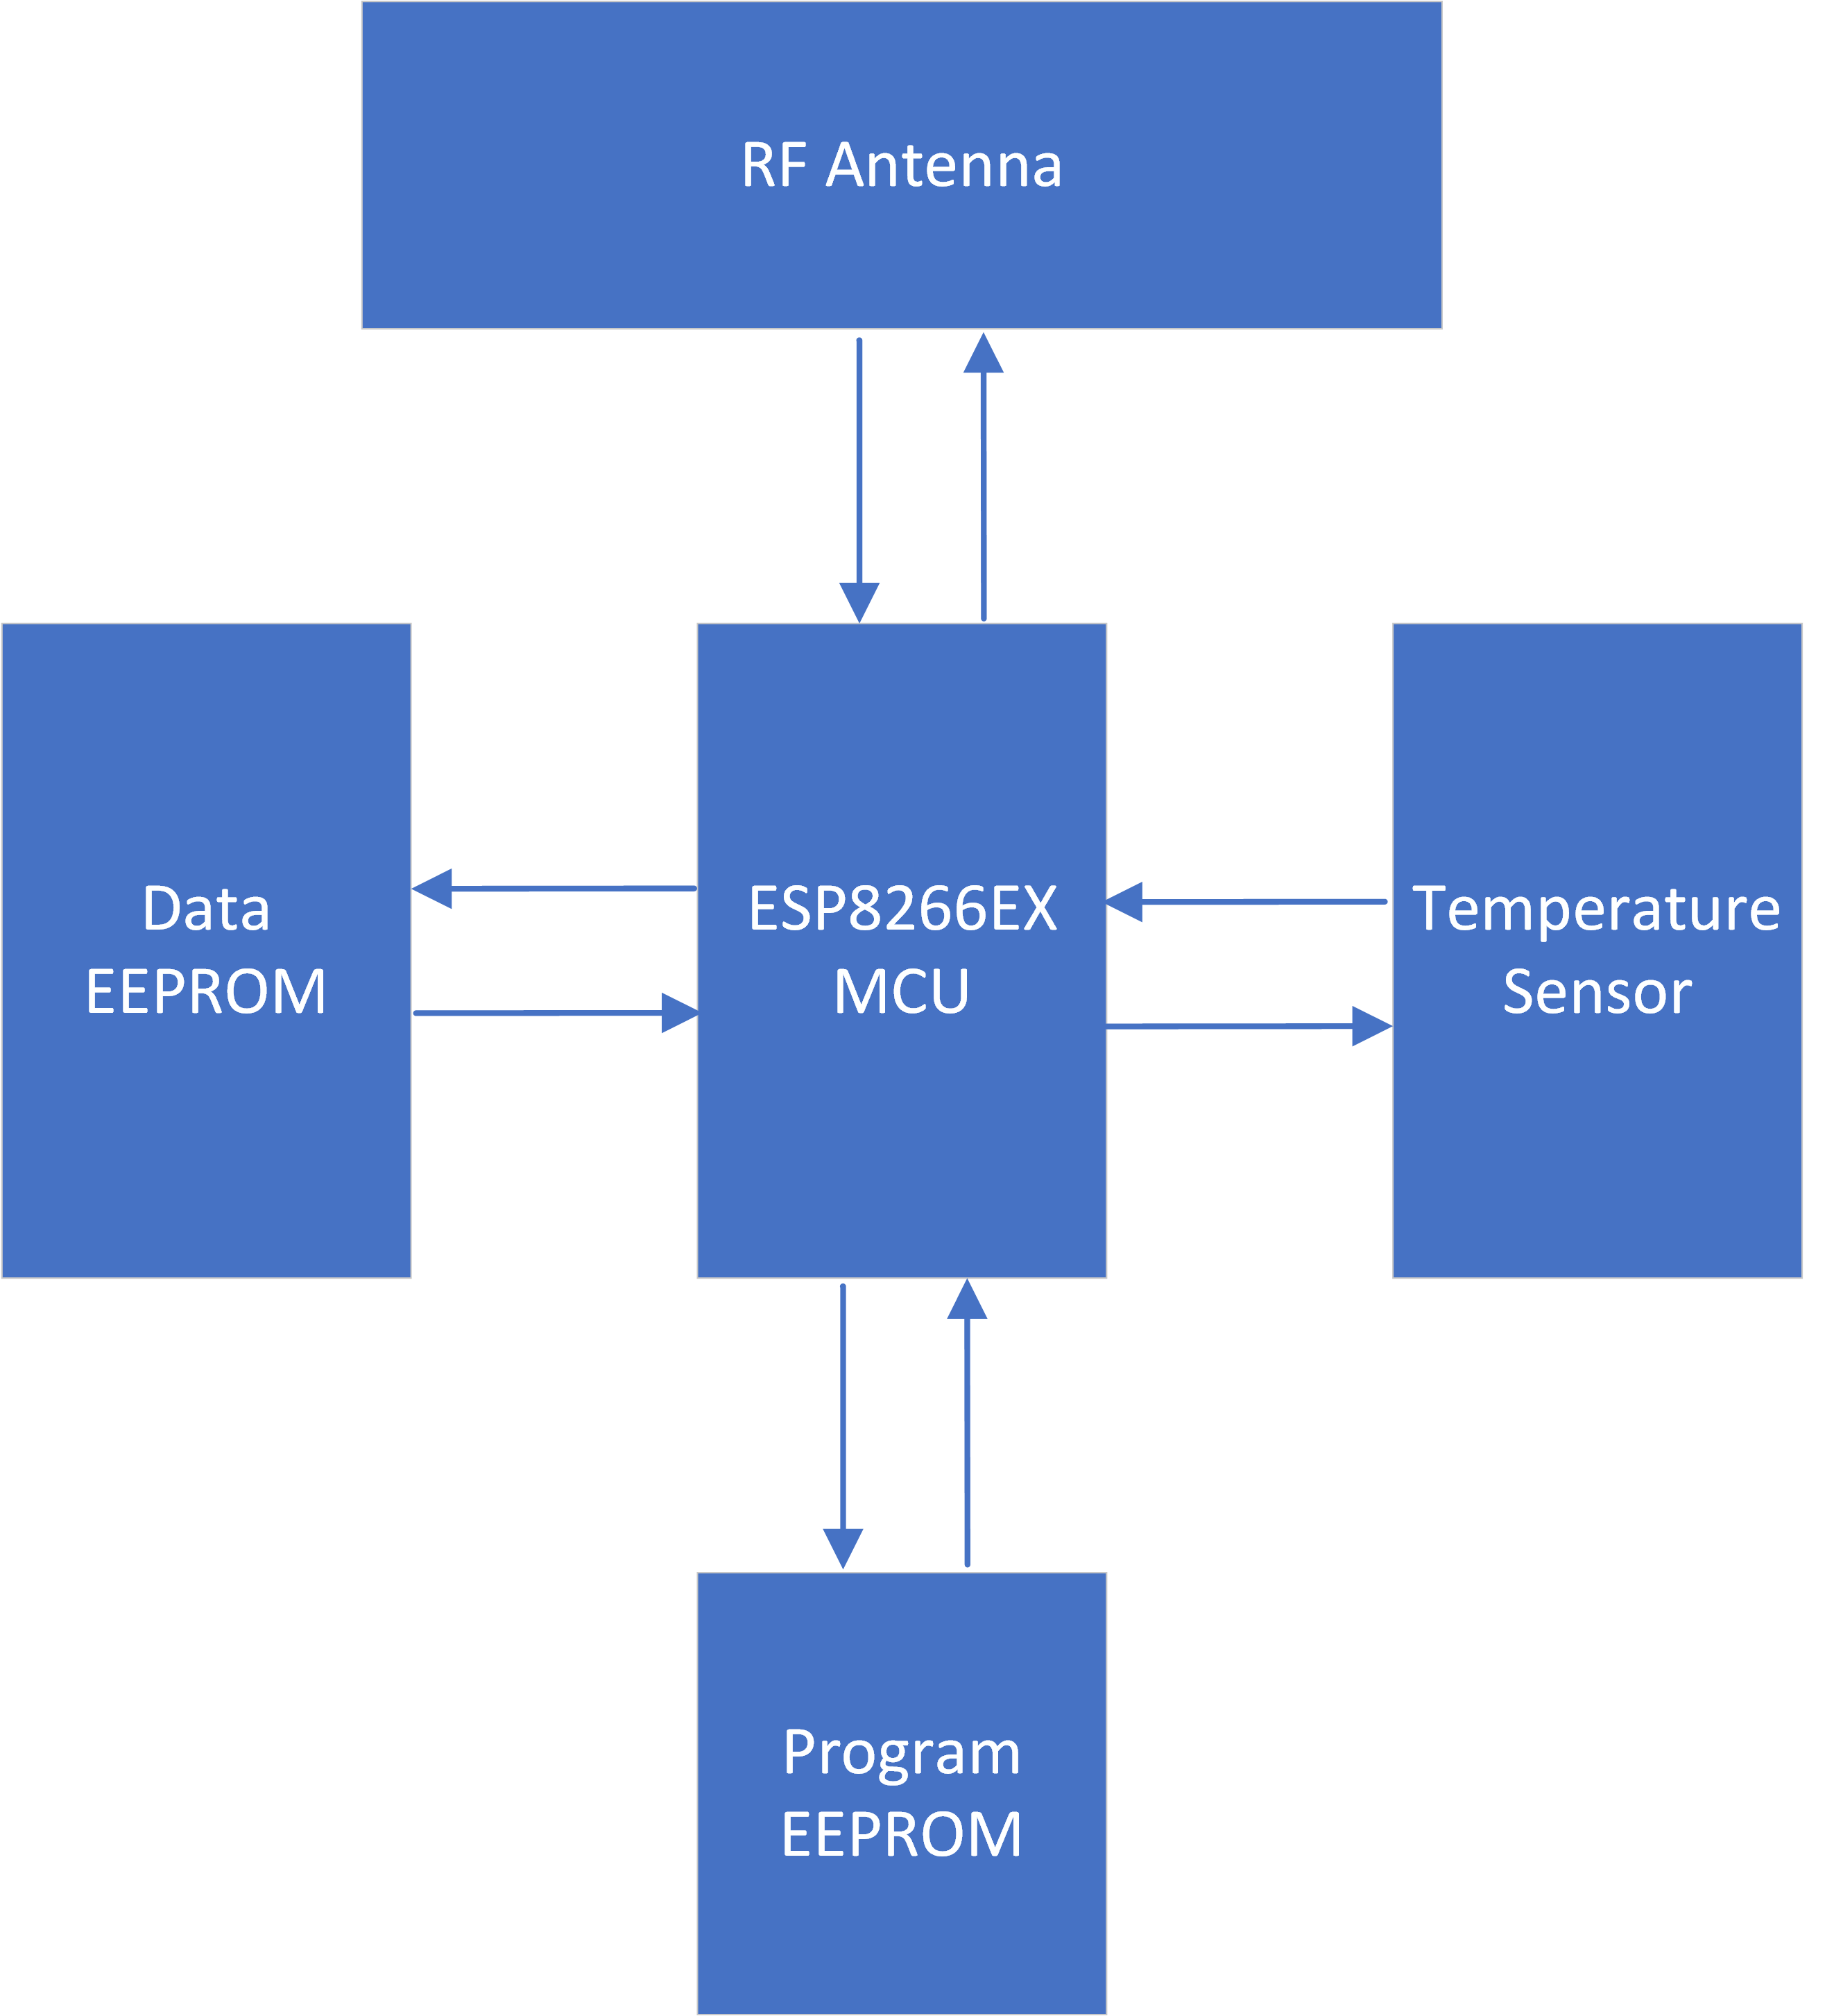
\includegraphics[scale = 0.8]{imagens/BD.png}
    \caption{\textbf{Device's block diagram}.}
    \label{02fig:BD}
\end{figure}


\subsection{Schematics}\label{02Sub:Schematics}

To further delve into the circuit's details, on Figure \ref{02fig:schematics-1} is the schematic diagram of the circuit. It is also divided into 
four blocks, each serving a specific purpose in the device's functionality as follows:

\begin{itemize}
    \item Power Supply Block: The power supply block provides a stable +3.3V voltage to the entire circuit. It ensures 
    that all components receive the necessary power to operate efficiently and reliably. The power supply block includes a 3.7V (mAh to be
    decidade, depending on the longevity needed) and a voltage regulators. Decoupling capacitors and other necessary components to regulate and 
    distribute power are cointained in the ``Main Circuitry'' (see Figure \ref{02fig:schematics-1}).

    \item Program and Data Memory Block: This block encompasses the program and data memories of the device. The program memory, 
    represented by the MX25R3235F chip, stores the firmware responsible for controlling the device's operations. The data memory, 
    represented by the AT25SF081 chip, stores collected data for future transmissions. This block includes the necessary 
    connections between the microcontroller and the memory chips.

    \item Temperature Sensing Block: The temperature sensing block includes the temperature sensor component (TMP35) and its 
    associated circuitry. The sensor measures the ambient temperature and then converts it temperature reading 
    into a eletctrical analog format for processing by the microcontroller. This block is responsible for accurate temperature measurement and 
    data acquisition.

    \item Main Block (Microcontroller and Components): The main block contains the microcontroller (ESP8266EX) and its associated
     components, in addition to the 2.4GHz RF antenna. The microcontroller serves as the central processing unit of the device, executing firmware 
     instructions and coordinating various operations. This block includes components such as crystal oscillators, capacitors, resistors and 
     inductors; these are the supporting elements necessary for the microcontroller's functionality.


\end{itemize}



These four blocks work together to ensure the device's proper operation. The power supply block provides the necessary voltage, 
the program, and data memory block stores and retrieves essential information, the temperature sensing block enables temperature 
measurement. Last but not least, the main block with the microcontroller controls and manages the device's overall functionality.


\begin{landscape}

\begin{figure}[H]
    \centering
    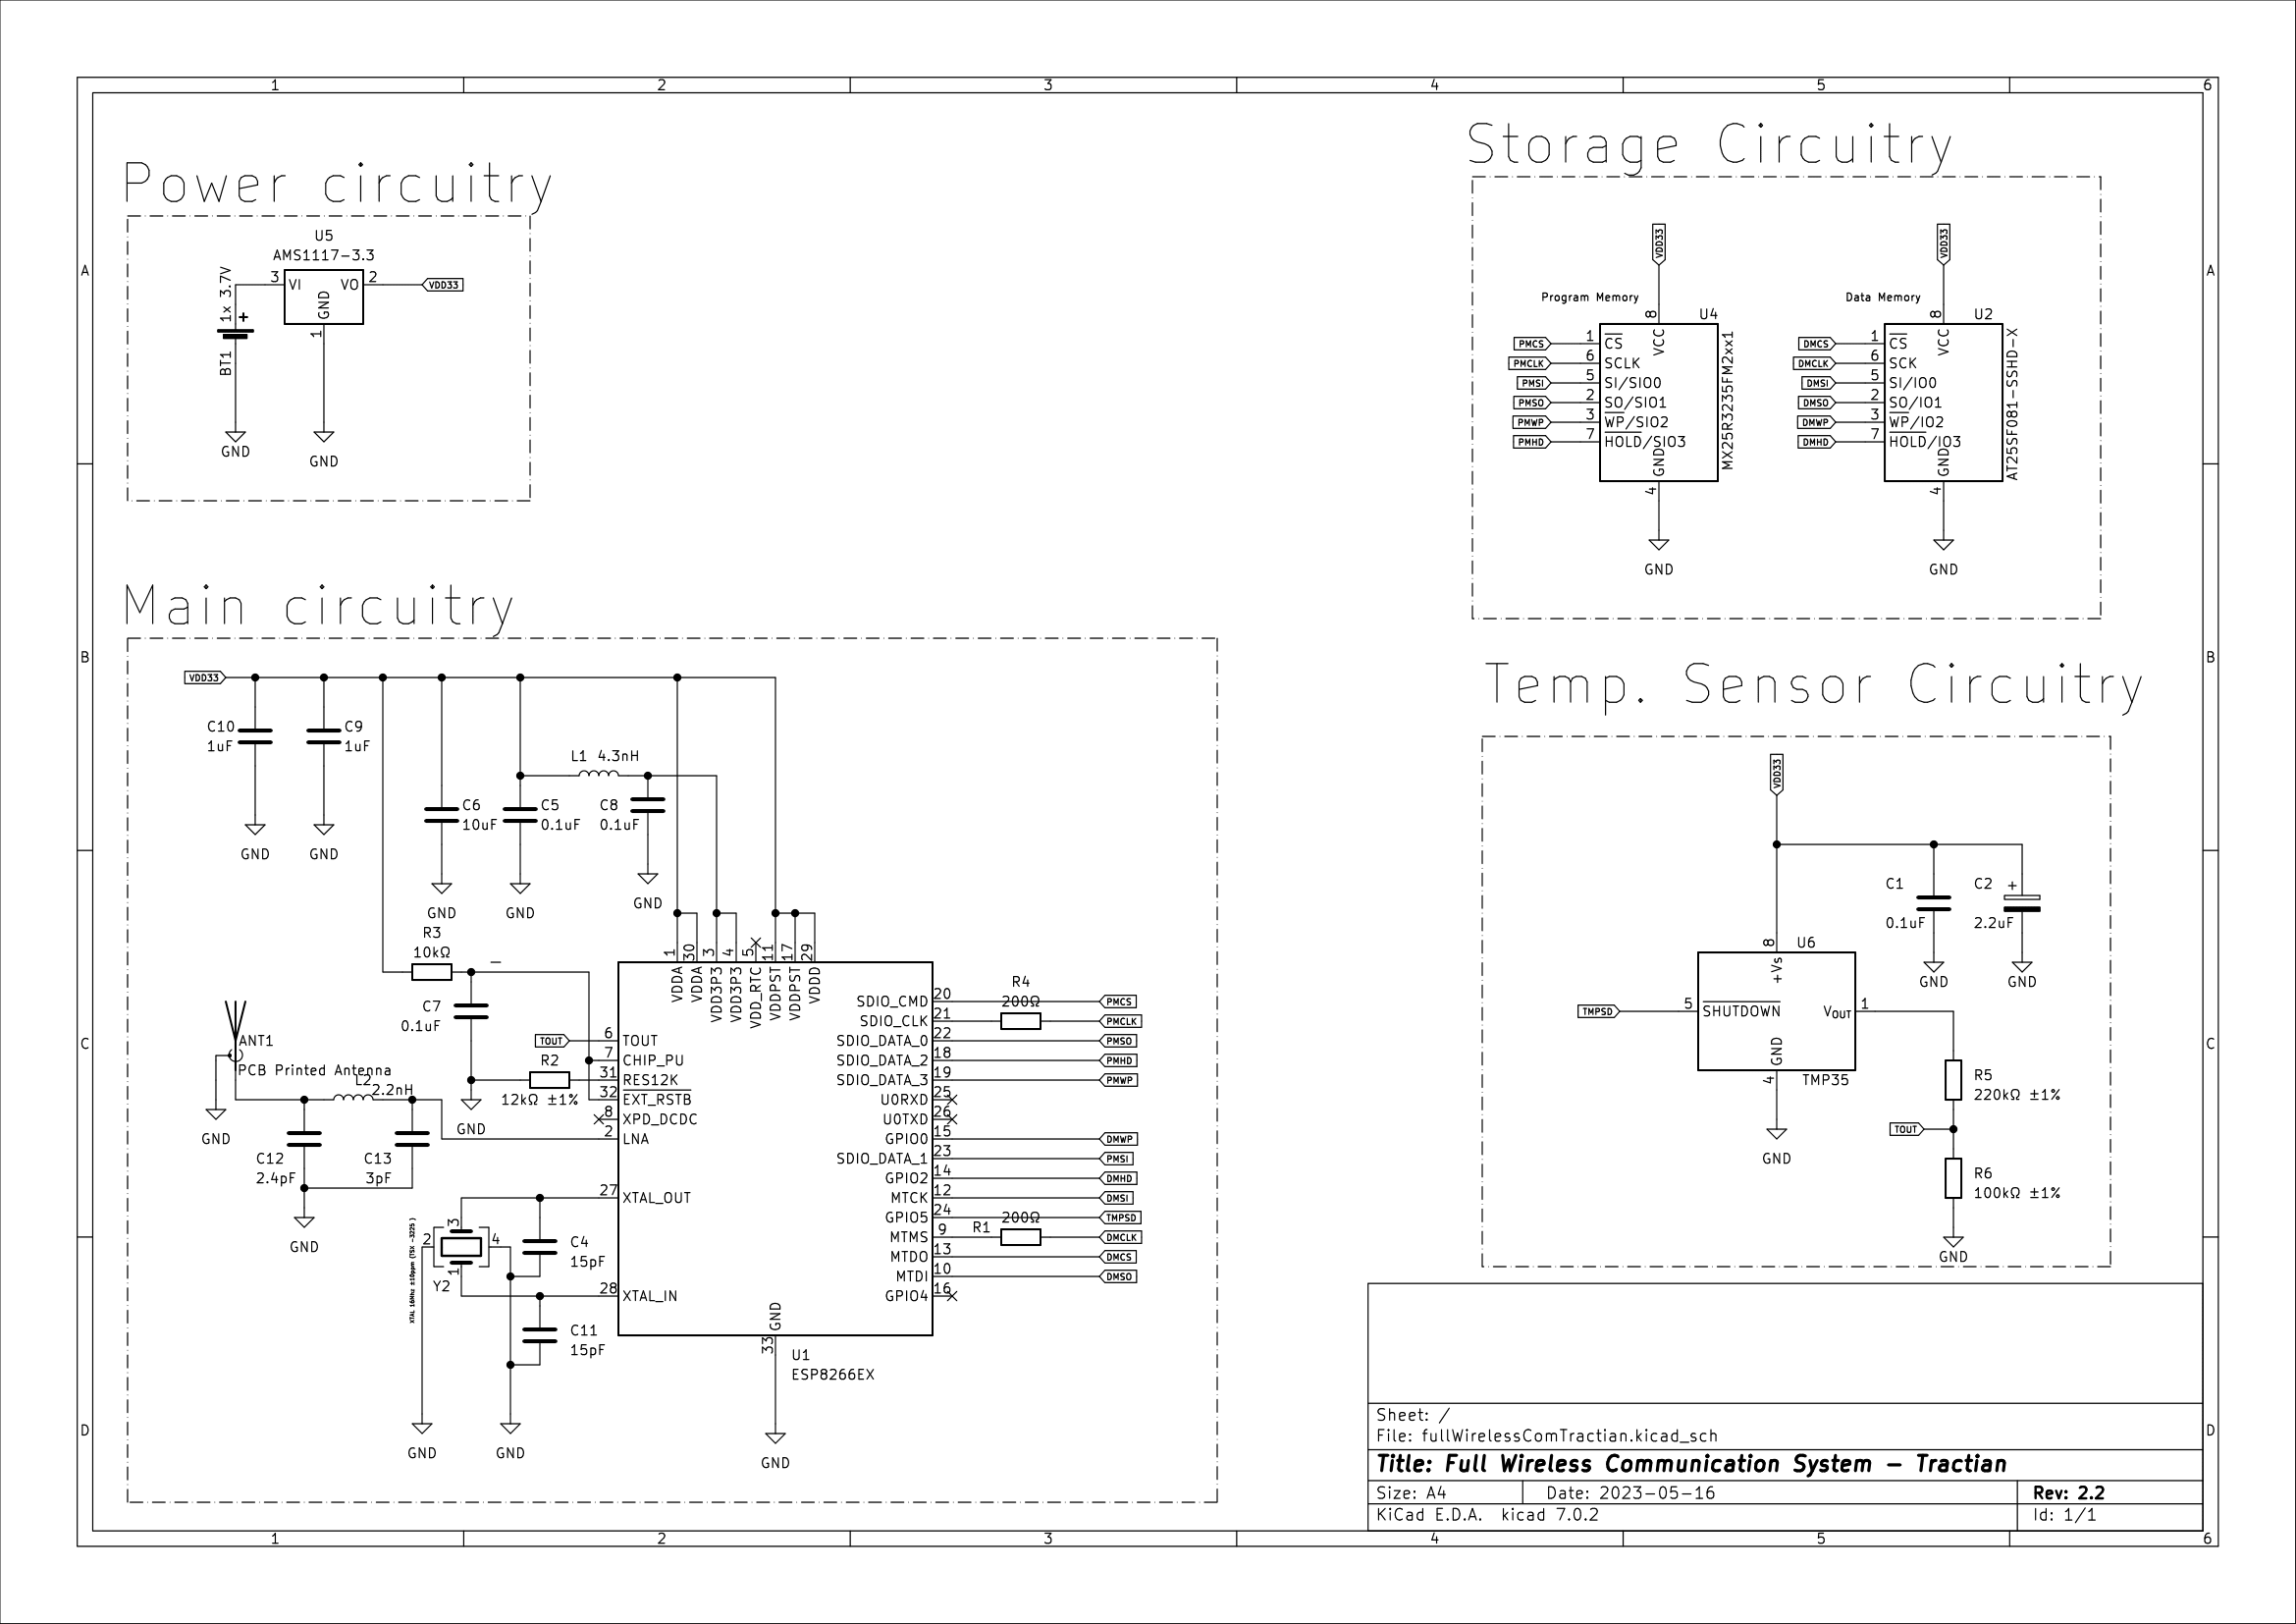
\includegraphics[scale = 0.775]{imagens/schematics-1.png}
    \caption{\textbf{Circuit Schematics}.}
    \label{02fig:schematics-1}
\end{figure}



\end{landscape}


\subsection{Circuit Diagrams}\label{02Sub:CircuitDiagrams}

We start highlitning the main points of the Main Circuitry, putting important
design requirements for the properly function of the ESP8266EX.

\subsubsection{Digital and Analog Supplies Circuitry}\label{02SubSub:DigitalAndAnalogSuppliesCircuitry}

For the analog power supply, ESP8266EX features five analog pins dedicated to power supply, encompassing Pin1, Pin3, and Pin4, 
which specifically cater to the power requirements of the internal PA and LNA. Furthermore, Pin29 and Pin30 serve as power inputs for the internal PLL. 
The acceptable voltage range for these analog power supply pins spans from 2.5 V to 3.6 V \cite{ESP8266HGL}.  \\ 

As for the digital power suplly, ESP8266EX is equipped with two digital pins, namely Pin11 and Pin17, 
dedicated to power supply. When it comes to the digital power supply, the inclusion of supplementary filter capacitors 
is unnecessary. The operational voltage range for the digital power supply pins spans from 1.8 V to 3.3 V \cite{ESP8266HGL}
Both Analog and Digital power supply connections can be seen on Figure \ref{02fig:analogAndDigitalSupplies1}

\begin{figure}[H]
    \centering
    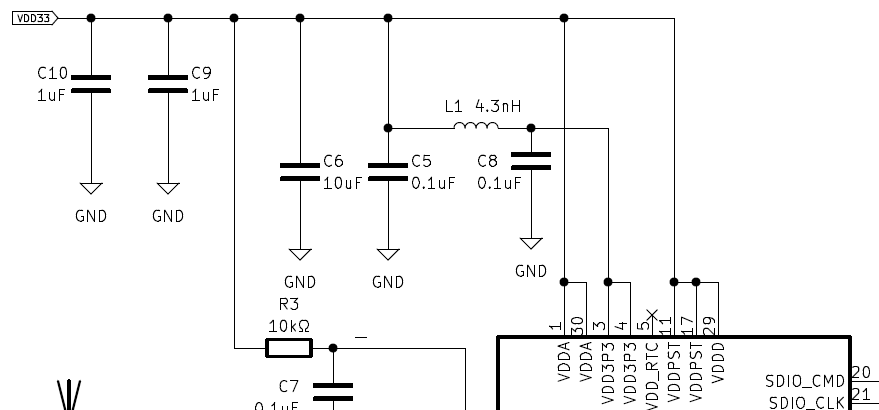
\includegraphics[scale = 0.775]{imagens/analogAndDigitalSupplies.png}
    \caption{\textbf{Digital and Analog Supplies Circuitry}.}
    \label{02fig:analogAndDigitalSupplies1}
\end{figure}



\subsubsection{RC Delay Reset Circuitry}\label{02SubSub:RCDelayResetCircuitry}


The reset pin of ESP8266EX is denoted as Pin32 EXT\_RSTB and plays a vital role in the device's 
operation \cite{ESP8266HGL}. This pin possesses an internal pullup resistor and operates on an active low mechanism. 
As for Pin7 CHIP\_EN, it functions as the enable pin for ESP8266EX. When held at a low state, ESP8266EX powers 
off \cite{ESP8266HGL}. Its connections can see on the Figure \ref{02SubSub:RCDelayResetCircuitry}
shwon in the section (\ref{02SubSub:12kOhmRes}) below.


\subsubsection{12Kohm RES}\label{02SubSub:12kOhmRes}

An external GND 12k$\Omega$ showed on Figure \ref{02SubSub:RCDelayResetCircuitry} resistor should be connected with the ERS12K pin 
(pin 31) \cite{ESP8266HGL}. This component must have high accuracy when controlling the bias current. For this,
a 12k$\Omega \pm 1\%$ is required.


\begin{figure}[H]
    \centering
    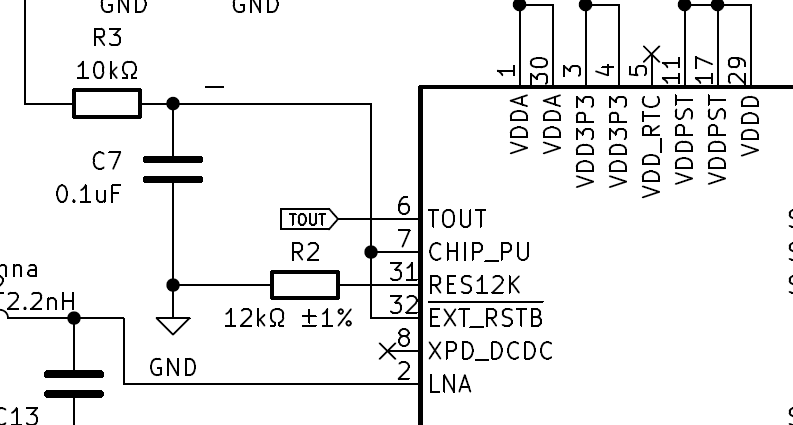
\includegraphics[scale = 0.5]{imagens/RCDelayResetCircuitry.png}
    \caption{\textbf{RC Delay Reset circuitry and 12K RES Pin}.}
    \label{02fig:RCDelayResetCircuitry}
\end{figure}


\subsubsection{RF Antenna Circuitry}\label{02SubSub:RFAntennaCircuitry}

For the 2.4Ghz RF antenna, in terms of ``abstract'' circuit itself, the only requirements is that the
the impedance at the output terminal of the ESP8266 PA is $39 + j6 \Omega$, which necessitates a corresponding 
matched impedance of $39-j6 \Omega$ (from the antenna to the chip). For such implementation,
see the Figure \ref{02fig:RFAntennaCircuitry} below.




\begin{figure}[H]
    \centering
    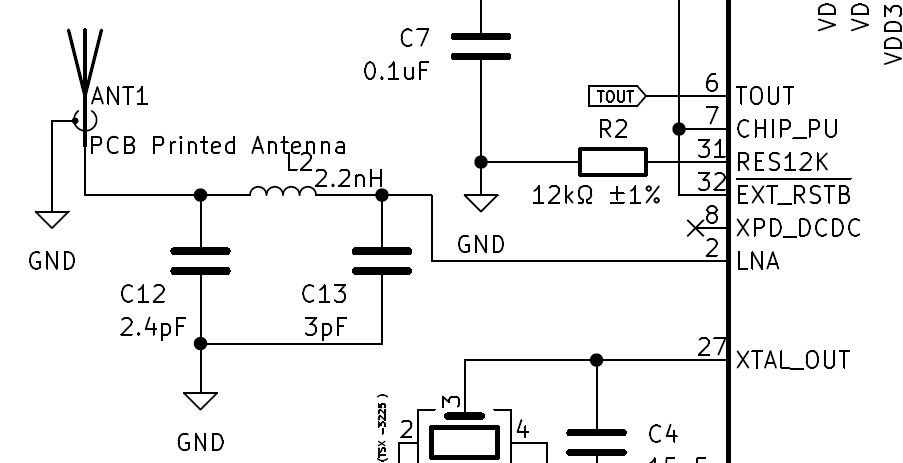
\includegraphics[scale = 0.5]{imagens/RFAntennaCircuitry.png}
    \caption{\textbf{2.4GHz Antenna circuitry}.}
    \label{02fig:RFAntennaCircuitry}
\end{figure}


\subsubsection{XTAL Circuitry}\label{02SubSub:XTALCircuitry}


\begin{figure}[H]
    \centering
    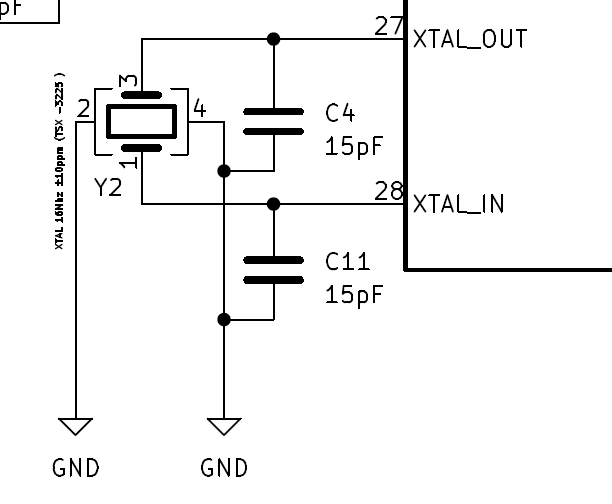
\includegraphics[scale = 0.5]{imagens/XTALCircuitry.png}
    \caption{\textbf{Crystal Oscillator Circuitry}.}
    \label{02fig:XTALCircuitry}
\end{figure}


\subsubsection{Drive Current Serial Clock RES}\label{02SubSub:DriveCurrentSerialClockRES}


\begin{figure}[H]
    \centering
    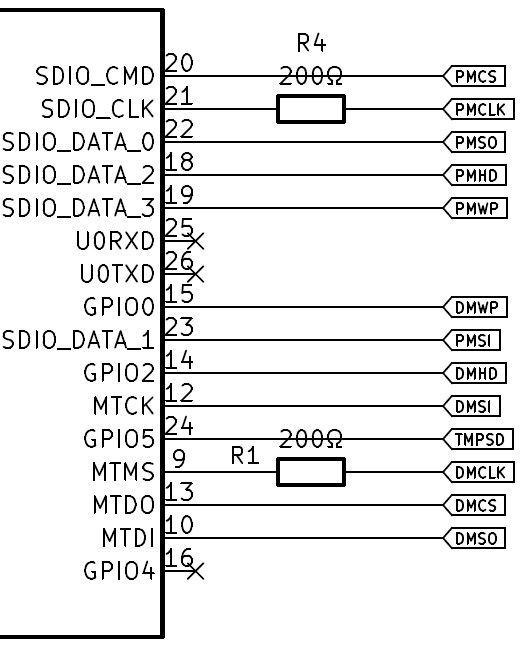
\includegraphics[scale = 0.5]{imagens/DriveCurrentSCLKRES.png}
    \caption{\textbf{200$\Omega$ RES Drive Current}.}
    \label{02fig:DriveCurrentSCLKRES}
\end{figure}




As for the Nets connected on each of the pins shown in Figure \ref{02fig:DriveCurrentSCLKRES},
``P'' stands for ``Program'', ``D'' is ``Data'', ``SI'' and ``SO'' are ``Serial IN'' (MOSI) and
``Serial Out'' (MISO) respectivily (notice the ``IN'' ``Out'' refers to the slave pins). Moreover,
``SCLK'' means ``Serial Clock'', ``WP'' is ``Write Protect', ``HD'' refers to ``Hold''.
Finnaly, ``TEMPSD'' stands for ``TMP 35 Shutdown''. So, for instance, ``DMCLK''
refers to the ``Data Memory Serial Clock'' Net. From this point, the rest of the 
blocks are described.





\subsubsection{Power Circuitry}\label{02SubSub:PowerCircuitry}

\begin{figure}[H]
    \centering
    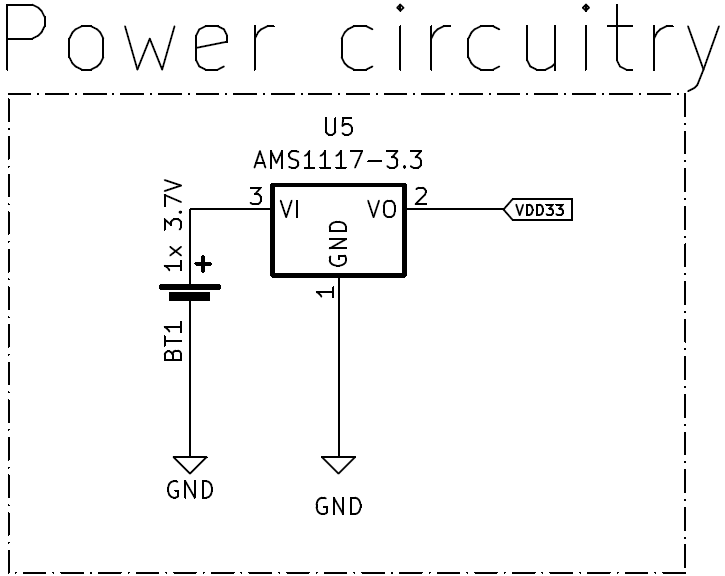
\includegraphics[scale = 0.5]{imagens/powerCircuitry.png}
    \caption{\textbf{3.3V Power circuitry}.}
    \label{02fig:powerCircuitry}
\end{figure}




\subsubsection{Storage Circuitry}\label{02SubSub:StorageCircuitry}

As for the program memory, since there is no internal memory available, an external flash memory is required for the ESP8266EX to store the user 
program. It is important to consider that the minimum capacity of the memory should be 512kB for disabled OTA (firmware updates Over The Air) or 1MB 
for enabled OTA. For firmware programming into the memory, the ESP8266EX supports Standard SPI, Dual SPI, and Quad SPI, which need to be selected prior 
to the programming process. The chosen memory, MX25R3235F \cite{ProgramMemoryMX}, meets all the aforementioned requirements. \\


For the data memory, the requirements essentially boil down to having sufficient space (min 500kB) and supporting SPI communication. The chosen IC, 
AT25SF081 \cite{DataMemoryAT}, fulfills these requirements. Additionally, this IC allows for serial data traffic on its I/Os at speeds of up to 50MHz 
(85MHz and 104MHz in specific cases). Since the communication with this chip was achieved through bit banging (see section \ref{04Sub:FeaturesAndAlgorithms}
), with an SCLK oscillation period of 6$\mu s$, \textit{i.e.}, a frequency of $f = $ 166.666kHz, operating with this chip is entirely feasible, obviating the 
need for hardware-based SPI interface. Furthermore, The protection bits are set to zero by default \cite{DataMemoryAT}, and there is no need to modify these bits. 
Therefore, the memory can be programmed and erased without any difficulties. Both program and data memory can be seen on Figure 
\ref{02fig:storageCircuitry}


\begin{figure}[H]
    \centering
    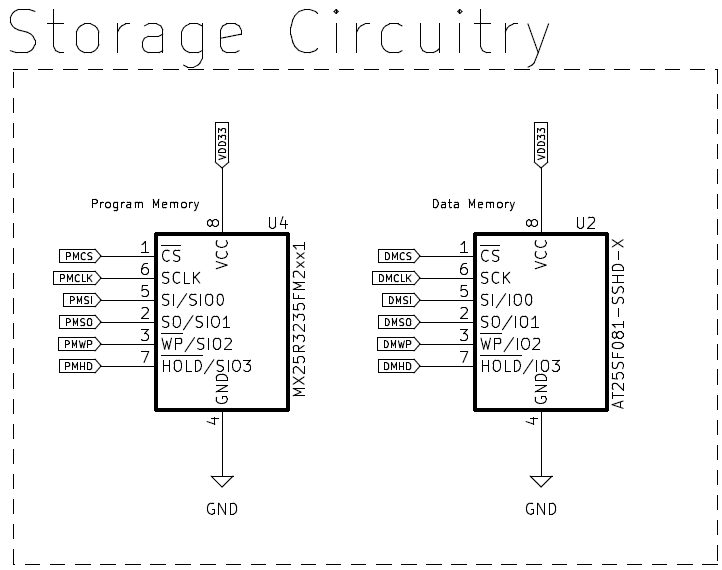
\includegraphics[scale = 0.6]{imagens/storageCircuitry.png}
    \caption{\textbf{Storage circuitry - Program and Data Memory}.}
    \label{02fig:storageCircuitry}
\end{figure}








\subsubsection{Temperature Sensor Circuitry}\label{02SubSub:TemperatureSensorCircuitry}




\begin{figure}[H]
    \centering
    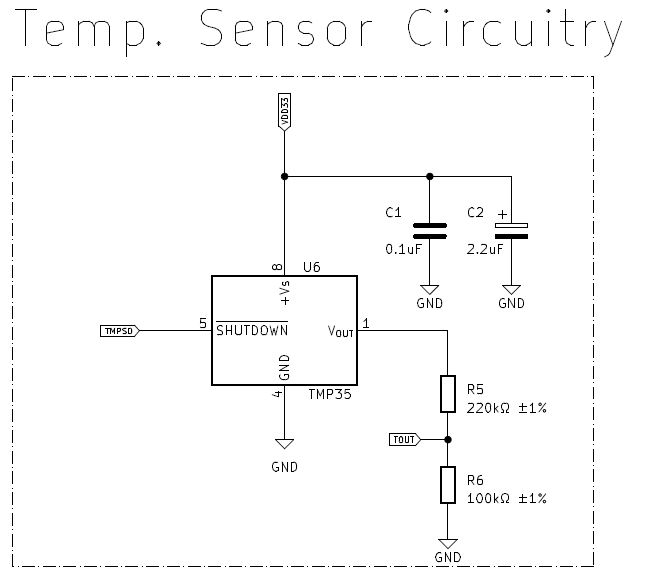
\includegraphics[scale = 0.6]{imagens/temperatureSensorCircuitry.png}
    \caption{\textbf{Temperature measuring circuitry}.}
    \label{02fig:temperatureSensorCircuitry}
\end{figure}



\subsection{Components}\label{02Sub:Components}


List of componentes, its values, packages, etc














%%%%%%%%%%%%%%%%%%%  END  %%%%%%%%%%%%%%%%%%%%
%%%%%%%%          Schematics          %%%%%%%%
%%%%%%%%%%%%%%%%%%%%%%%%%%%%%%%%%%%%%%%%%%%%%%